% ****** Start of file apssamp.tex ******
%
%   This file is part of the APS files in the REVTeX 4 distribution.
%   Version 4.0 of REVTeX, August 2001
%
%   Copyright (c) 2001 The American Physical Society.
%
%   See the REVTeX 4 README file for restrictions and more information.
%
% TeX'ing this file requires that you have AMS-LaTeX 2.0 installed
% as well as the rest of the prerequisites for REVTeX 4.0
%
% See the REVTeX 4 README file
% It also requires running BibTeX. The commands are as follows:
%
%  1)  latex apssamp.tex
%  2)  bibtex apssamp
%  3)  latex apssamp.tex
%  4)  latex apssamp.tex
%
\documentclass[prb,aps,twocolumn,preprintnumbers,amsmath,amssymb]{revtex4}
%\documentclass[preprint,showpacs,preprintnumbers,amsmath,amssymb]{revtex4}

% Some other (several out of many) possibilities
%\documentclass[preprint,aps]{revtex4}
%\documentclass[preprint,aps,draft]{revtex4}
%\documentclass[prb,twocolumn,showpacs,preprintnumbers,amsmath,amssymb]{revtex4}% Physical Review B

\usepackage{graphicx}% Include figure files
\usepackage{dcolumn}% Align table columns on decimal point
\usepackage{bm}% bold math
\usepackage[utf8]{inputenc}
\newcommand*{\Scale}[2][4]{\scalebox{#1}{$#2$}}%
%\nofiles

\begin{document}

\title{Osciloscopio}% Force line breaks with \\

\author{Alejandro Hernández A.}%
 \email{a.hernandez105@uniandes.edu.co}
\author{Daniel Sánchez M.}%
 \email{d.sanches462@uniandes.edu.co}
\affiliation{%
Departamento de Física\\ Universidad de los Andes, Bogotá, Colombia.\\
}%
\date{3 de septiembre de 2015\\}% It is always \today, today,
             %  but any date may be explicitly specified

\begin{abstract}
Este informe presenta los datos obtenidos al medir voltaje y corriente para configuraciones solicitadas de circuitos RC y RLC. Para el circuito RC, se determinó el tiempo característico de carga y descarga del condensador, y se otuvieron los siguientes datos: $\tau_{carga} = $ con error porcentual $E\% = \%$ y $\tau_{descarga} = $ con error porcentual $E\% = \%$. Para el circuito RLC, se determinó la frecuencia natural del sistema y el parámetro de resistencia y los datos obtenidos fueron los siguientes: $f_{0} = $ con error porcentual $E\% = \%$ y $\gamma = $ con error porcentual $E\% = \%$. 
\\

%\smallskip
\noindent \textbf{Conceptos clave:} Circuito RC, circuito RLC, oscilador amortiguado.
\end{abstract}
                             
\maketitle

\section{\label{sec:level1}Introducción.}

Las resistencias, condensadores e inductancias son algunos de los elementos electrónicos de dos terminales más usados en diversos dispositivos tegnológicos de la actualidad. Y dado a que la implementación de los circuitos que usan estos elementos es relativamente simple, las características experimentales de estos elementos pueden ser estudiadas rigurosamente, ya sea con corriente directa DC o con corriente alterna AC.\\

En este circuito no interesan los circuitos RC y RLC, ambos en serie, cuyas principales características se presentan a continuación.

\subsection{Circuito RC}

El circuito a usar se muestra en la figura \ref{fig: RC}

\begin{figure}[h!]
	\centering
	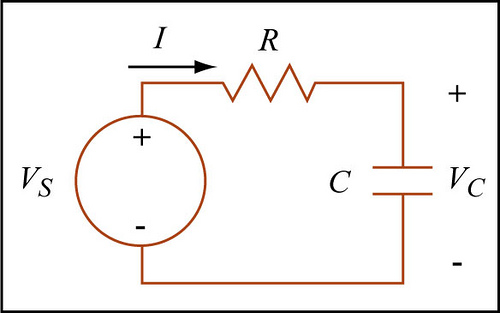
\includegraphics[width=0.4\textwidth]{RC}
	\caption{Circuito RC en serie}
	\label{fig: RC}
\end{figure} 

Para el proceso de carga del condensador, el voltaje a través de la resistencia viene dado por \eqref{VRC}.

\begin{equation}
\label{VRC}
V_{r} = V_{f}e^{-\frac{t}{RC}}
\end{equation}

Donde $V_{f}$ es el voltaje de la fuente (voltaje final del condensador).\\

Para el proceso de descarga el voltaje de la resistencia está dado por \eqref{RC}.

\begin{equation}
\label{RC}
V_{r} = -V_{0}e^{-\frac{t}{RC}}
\end{equation}

Donde $V_{0}$ representa el voltaje inicial del condensador.\\

En las ecuaciones anteriores la constante $\tau = RC$ tiene unidades de tiempo y corresponde al tiempo característico de carga o descarga del condensador de acuerdo a la situación de interés. Para el proceso de carga. Dicha constante es interpretada como el tiempo que tarda en cargarse (o descargarse) el condensador a un $67\%$ de su carga máxima.\\

Ahora bien, el circuito RLC a usar se muestra en la figura \ref{fig: RLC}

\begin{figure}[h!]
	\centering
	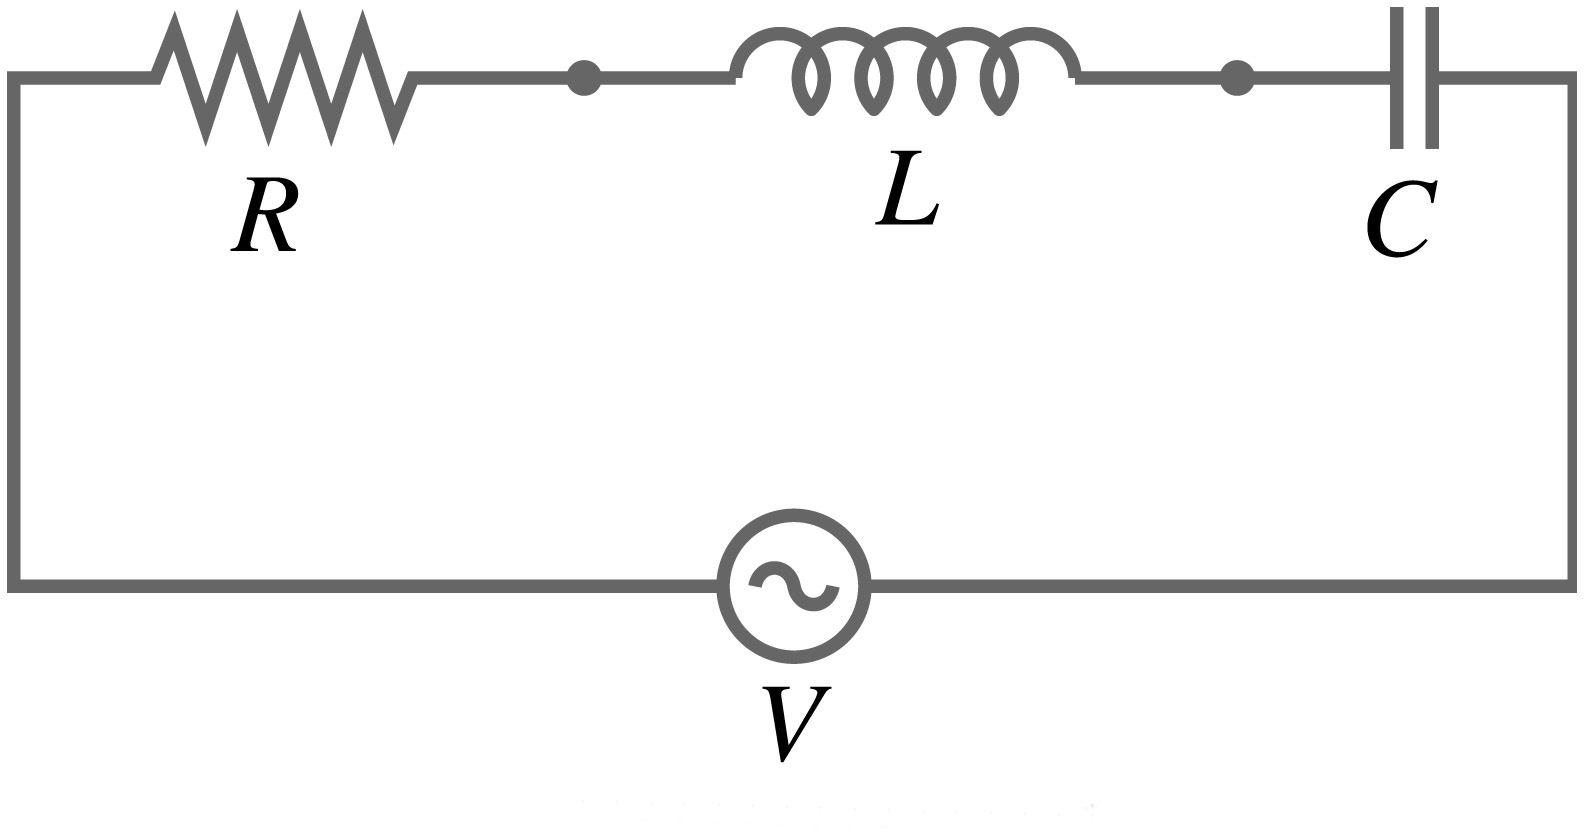
\includegraphics[width=0.4\textwidth]{RLC}
	\caption{Circuito RLC en serie}
	\label{fig: RLC}
\end{figure}

Este circuito es caracterizado por la ecuación \eqref{RLC}.

\begin{equation}
\label{RLC}
\frac{d^2 q}{d t^2} + \frac{R}{L}\frac{d q}{d t} + \frac{1}{LC}q = V(t)
\end{equation}

Donde $V(t)$ es el voltaje de la fuente, $\gamma = \frac{R}{L}$ es el factor análogo a la fricción en sistemas mecánicos que da cuenta de la disipación de energía en la resistencia, y $\omega_{0}^2 = \frac{1}{LC}$ es la frecuencia natural del sistema.\\

Suponiendo $V = \frac{V_{0}}{L} e^{i\omega t}$, el sistema está forzado y $\omega$ es la frecuencia de forzamiento y los parámetros $\gamma$ y $\omega_{0}$ determinan la resonancia del sistema con respecto al forzamiento  y determinan la existencia o no de soluciones oscilatorias cuando $\omega = 0$. Para dicha dependencia temporal del voltaje, la solución no homogénea de la ecuación \eqref{RLC} tiene la forma $q(t) = A(\omega) e^{i \omega t}$, con la amplitud dada por la ecuación \eqref{amplitud}.

\begin{equation}
\label{amplitud}
A(\omega) = \frac{V_{0}}{L}\frac{1}{\sqrt{(\omega^2 - \omega_{0}^2)^2+(\gamma \omega)^2}}
\end{equation}

Y la frecuencia de resonancia (frecuencia en la que la amplitud es máxima) está dada por la ecuación \eqref{resonancia}.

\begin{equation}
\label{resonancia}
\omega_{res} = \sqrt{\omega_{0}^2 - \frac{\gamma^2}{4}}
\end{equation}

Allende de lo anterior, es preciso hablar de las figuras de Lissajous, ya que serán mencionadas en secciones posteriores de este informe. Las figuras de Lissajous son gráficas de un sistema con ecuaciones paramétricas dadas por:

\begin{equation}
\label{lissa}
\begin{split}
x &= A_{x}\sin(\omega_{x}t + \delta)\\
y &= A_{y}\sin(\omega_{y}t)
\end{split}
\end{equation}

Cabe mencionar que las condición para poder obtener figuras de Lissajous cerradas es que las frecuencias de las dos ondas superpuestas sean conmensurables, es decir, que sean números racionales. La visualización de estas curvas en un osciloscopio permiten verificar experimentalmente las cualidades teóricas de las superposición de en x y y de ondas producidas por un generador de señales.

\section{Montaje experimental}

Los instrumentos usados durante la práctica de laboratorio fueron un osciloscopio, dos generadores de señales, y diversos elementos electrónicos de dos terminales tales como resistencias, inductancias y condensadores.\\

El ocsilador y los generadores de señales se muestran en las figuras \ref{fig: osci} y \ref{fig: genr}

\begin{figure}[h!]
	\centering
	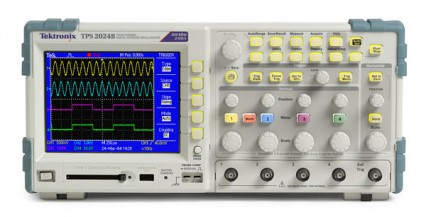
\includegraphics[width=0.4\textwidth]{osciloscopio}
	\caption{Ociloscopio usado para la toma de datos}
	\label{fig: osci}
\end{figure}

\begin{figure}[h!]
	\centering
	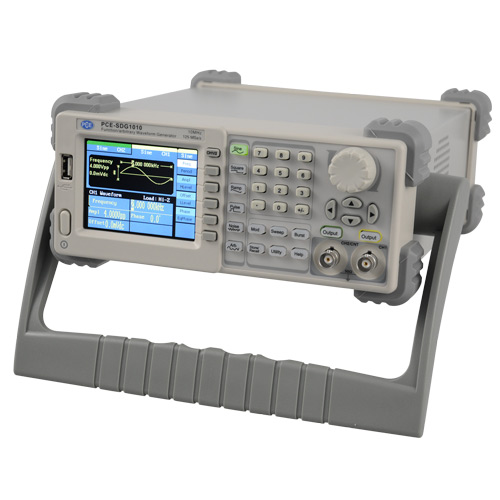
\includegraphics[width=0.4\textwidth]{generador}
	\caption{Generador de señales usado en la practica.}
	\label{fig: RLC}
\end{figure}

\section{Resultados y análisis}

Los resultados de las mediciones de corriente y voltaje se muestran en la Tabla \ref{Tabla 1}.\\

\begin{table}[h!]
	\caption{\label{Tabla 1}Voltaje y corriente para.}
	\begin{ruledtabular}
		\begin{tabular}{ccccc}
			\multicolumn{1}{c}{$V \pm 1V$} & \multicolumn{4}{c}{$A \pm 0.01A$ } \\
			\hline
			Voltaje &$I_{2\ cm}$&$I_{3\ cm}$&$I_{4\ cm}$&$I_{5\ cm}$\\
			\hline
			110 & 2.60 & 1.44 & 1.11 & 0.85 \\
			120 & 2.73 & 1.73 & 1.21 & 0.92\\
			130 & 2.79 & 1.17 & 1.30 & 0.96\\
			140 & 2.83 & 1.86 & 1.35 & 1.02\\
			150 & 2.96 & 1.87 & 1.39 & 1.08\\
			160 & 3.06 & 1.99 & 1.41 & 1.13\\
			170 & 3.17 & 2.03 & 1.47 & 1.17\\
			180 & 3.28 & 2.09 & 1.53 & 1.22\\
			190 & 3.38 & 2.15 & 1.58 & 1.25\\
			200 & 3.46 & 2.21 & 1.63 & 1.30\\
			210 & 3.60 & 2.28 & 1.68 & 1.33\\
			220 & 3.68 & 2.33 & 1.72 & 1.36\\
			230 & 3.73 & 2.40 & 1.77 & 1.40\\
			240 & 3.79 & 2.46 & 1.81 & 1.43\\
			250 & 3.90 & 2.50 & 1.84 & 1.46\\
			260 & 3.98 & 2.56 & 1.89 & 1.49\\
			270 & 4.05 & 2.62 & 1.93 & 1.53\\
		\end{tabular}
	\end{ruledtabular}
\end{table}

Con el fin de analizar los datos, es conveniente ver \eqref{carga-masa} de la siguiente manera:

\begin{equation}
V = \frac{e}{m_{e}}\cdot\frac{(Br)^2}{2} 
\label{lineal}
\end{equation}

Identificando $\frac{(Br)^2}{2} \rightarrow x$ y $V \rightarrow y$, se puede ver en la figura \ref{fig:lineal} que los datos efectivamente satisfacen la relación dada por \eqref{lineal}, razón por la cual se justifica hacer una regresión lineal de los datos.\\


Con lo anterior, se obtiene el siguiente valor para la carga específica del electrón:

\begin{equation}
\left( \frac{e}{m_{e}} \right)_{exp} = (1.550 \pm 0.050) \cdot 10^{11} \frac{C}{kg} 
\end{equation}

Con una correlación de $r^2 = 0.935$ y error estándar de $s = 50.020 \cdot 10^{9}$. Y al comparar con el valor teórico\footnote{Valor obtenido de https://en.wikipedia.org/wiki/Mass-to-charge\_ratio} de dicha constante, $\left( \frac{e}{m_{e}} \right)_{teo} = (1.758 \cdot 10^{11}  \pm 39)  \frac{C}{kg}$, el cálculo del error porcentual arroja un resultado de $E\% = 11.831\%$.\\

Es preciso mencionar que hubo múltiples factores que generaron dicho error, entre ellos destacan los siguientes:

\begin{itemize}
	\item Se observó que los datos de corriente y voltaje que generaban una determinada curvatura del haz de electrones variaban mucho estando cerca de los radios marcados en el \textit{narrow beam tube}, y dado a que se requería que el haz pasara justo por encima de las marcas, consideramos que esta difucltad fue la que causó el error sistemático más significativo del experimento.
	
	\item Además de lo mencionado anteriormente, fue difícil ajustar el \textit{narrow beam tube} de tal forma que solo se observara un círculo y no una espiral como trayectoria del haz de electrones, complicando de esta manera la realización de medidas completamente satisfactorias.
\end{itemize}
	
Continuando con los errores que ocurrieron durante e laboratorio, es preciso hablar de la forma en la que se calculó el campo magnético inducido. Para poder obtener una expresión para el campo, se asumió que la órbita del haz de eletrones estaba ubicada justamente en el centro de las espiras y, por tanto, experimentaba un campo magnético dado por \eqref{campo helm.} sobre todos los puntos de la trayectoria del haz. Sin embargo, la órbita no coincidía exactamente con el centro del círculo y por ende, el campo magnético estaba dado por la expresión dada para $B_{z}$ con $z \neq 0$. En adición a lo anterior, dado que $\frac{dB_{z}}{dz} \neq 0$ para $z \neq 0$, esto indica que si bien el campo varía poco en la vecidad de $z = 0$, dicho campo no es uniforme y sería preciso considerar sus variaciones en en análisis de datos con el fin de obtener medidas más confiables.\\  


Análogamente, para la simplificación del cálculo de la fuerza de Lorentz se asumió que el campo cruzaba el plano vertical definido por el haz a un ángulo exacto $ \pi /2 $. Claramente, el hecho de que no se tengan en cuenta pequeñas variaciones de este ángulo pudo producir desviaciones que, aunque minúsculas, vale la pena mencionar. \\

También hay que tener en cuenta que , en las mediciones realizadas, se está despreciando completamente el campo magnético de la Tierra, el cual oscila entre ($25-75 \mu T$), apenas un orden de magnitud más pequeño que el de los campos manéticos generados por las bobinas de Helmholtz para los radios más grandes ($4$ y $5$ cm) los cuales se encuentran entre los $500$ y los $1000 \mu T$ para valores bajos de potencial. Todo esto fortalece aún más la idea de que la estimación realizada más confiable es la que corresponde al anillo de radio $2cm$ el cual  es el menos distorsionado por el campo magnético terrestre debido a que para formar un anillo de este tamaño se necesita un campo magnético bastante fuerte ( Entre $1$ y $2 mT$). Esto nos muestra que si el experimento se realiza con el haz de electrones paralelo al campo magnético terrestre se podría obtener una medición más confiable de los datos obtenidos, especialmente de aquellos cuyo radio es más grande. \\

Por último , vale la pena destacar la gran magnitud que tiene esta constante, especialmente comparada con la carga especíca del proton cuyo valor es aproximadamente $9.578 \cdot 10^7 C/kg$, cuatro ordenes de magnitud menor a la carga específica del electrón, hecho que fue determinante para establecer la existencia de dos tipos de partículas cargadas dentro del átomo, una de ellas de masa mil veces menor que la otra.\\


\section{Conclusiones}

\begin{itemize}
	
	\item El valor experimental obtenido para la carga específica del electrón $\left( \frac{e}{m_{e}} \right)_{exp} = (1.631 \pm 0.041) \cdot 10^{11} \frac{C}{kg}$ no es muy exacto dado a que el error porcentual de la medida fue de $E\% = 10.104\%$.
		
	\item La observación realizada de esta carga específica permite validar experimentalmente la idea acerca de la divisibilidad del átomo y su composición de partículas de carga tanto positiva como negativa, cuyas cargas se compensan perfectamente para formar un átomo neutro.
	
	\item Si bien se obtuvieron buenos resultados, es importante resaltar que tanto la intensidad de las trayectorias observadas, como el grosor de las mismas y la dificultad para ver círculos y no espirales, da pie para pensar acerca de la realización de medidas con instrumentos de mayor resolución con el fin de obtener mediciones más exactas de la razón carga masa.
	
\end{itemize}

\begin{thebibliography}{99}
\bibitem{eisberg} R. Eisberg, {\it Quantum Physics of Atoms, Molecules, Solids, Nuclei and Particles}{John Wiley \& Sons, USA, 1985}.\\

\bibitem{Tipler} Tipler, Paul A., \textit{Physics for scientists and engineers}. W.H. Freeman, 4 Edici\' on, 1999.\\
\bibitem{Taylor} Taylor, J.R., \textit{An Introduction to Error Analysis}. University Science Books, Sausalito, California. 2nd edition, 1982.\\
\bibitem{Guia} Phywe. Specific Charge of the Electron -e/m. 5.1.02-00\\
\end{thebibliography}

\end{document}
%
% ****** End of file apssamp.tex ******
